%**********************************************************
\myparagraph{CLocalSystem Methods}

The class constructor is shown in figure \ref{fig:CLocalSystemConstructor}. This is responsible for initializing all synchronization tools and private variables used, as well as creating the tasks \textit{tLoraRecv}, \textit{tRecvSensors} and \textit{tParkDetection}.

\begin{figure}[H]
	\centering
	%	\includegraphics[width=.3\textwidth]{09sw_specification/LS/clocalsystem/constructor}
	\caption{Flowchart: CLocalSystem constructor.}
	\label{fig:CLocalSystemConstructor}
\end{figure}

%******************************
The method \textit{run()}, presented in figure \ref{fig:CLocalSystemRun}, it's implemented similarly in various classes. This is responsible for starting timers that trigger the execution of tasks, and wait (\textit{join}) for the termination of the tasks.

\begin{figure}[H]
	\centering
	%	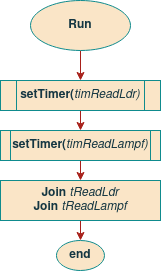
\includegraphics[width=.3\textwidth]{09sw_specification/LS/clocalsystem/run}
	\caption{Flowchart: CLocalSystem Run method.}
	\label{fig:CLocalSystemRun}
\end{figure}

%******************************
In figure \ref{fig:CLocalSystemtLoraRecv} is presented the task responsible for receiving a message from the gateway, via LoRa communication, parse it and execute the respective command.

\begin{figure}[H]
	\centering
	%	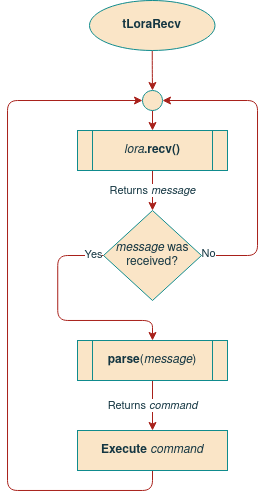
\includegraphics[width=.3\textwidth]{09sw_specification/LS/clocalsystem/tlorarecv}
	\caption{Flowchart: CLocalSystem tLoraRecv method.}
	\label{fig:CLocalSystemtLoraRecv}
\end{figure}

%******************************
In figure \ref{fig:CLocalSystemtRecvSensors} is presented the task responsible for receiving messages from the sensors daemon, via message queue. When there are no messages to read from the message queue, the task goes to sleep and is awaken when \textit{condRecvSensors} is notified. This happens in the \textit{sigHandler}, presented in figure \ref{fig:CLocalSystemsigHandler}, which is the signal handler for the main process, being this in charge of signaling the condition variable \textit{condRecvSensors} when a \textit{SIGUSR1} signal is catched.

\begin{figure}[H]
	\centering
	%	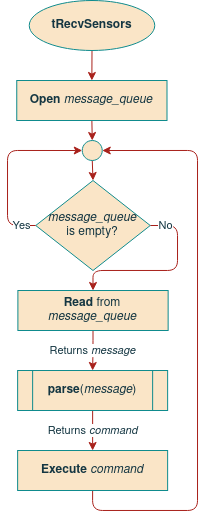
\includegraphics[width=.3\textwidth]{09sw_specification/LS/clocalsystem/trecvsensors}
	\caption{Flowchart: CLocalSystem tRecvSensors method.}
	\label{fig:CLocalSystemtRecvSensors}
\end{figure}

\begin{figure}[H]
	\centering
	%	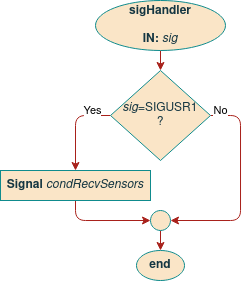
\includegraphics[width=.3\textwidth]{09sw_specification/LS/clocalsystem/sighandler}
	\caption{Flowchart: CLocalSystem sigHandler method.}
	\label{fig:CLocalSystemsigHandler}
\end{figure}

%******************************
This task, figure \ref{fig:CLocalSystemtParkDetection}, is responsible for using the \textit{camera} object, from \textit{CCamera}, and the \textit{park} object, from \textit{CParkDetection}, in order to capture image frames and process them, calculating the number of available spaces in the parking detected. This task is periodically awaken by the use of a timer, signaling the condition variable \textit{condCamFrame}.

\begin{figure}[H]
	\centering
	%	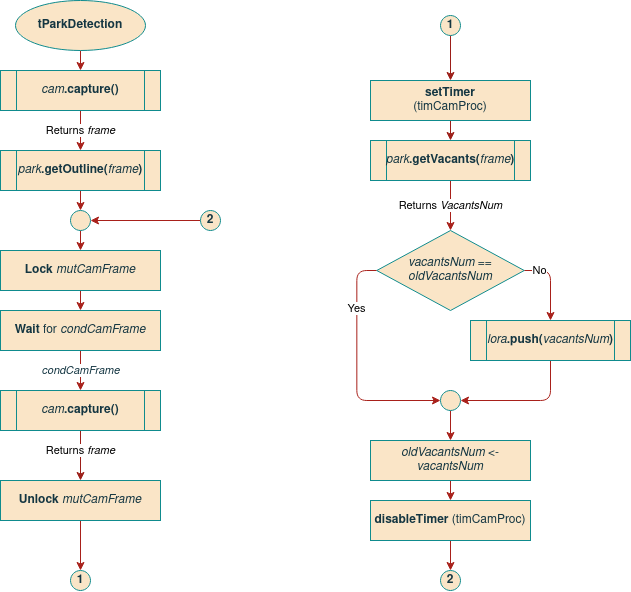
\includegraphics[width=.3\textwidth]{09sw_specification/LS/clocalsystem/tparkdetection}
	\caption{Flowchart: CLocalSystem tParkDetection method.}
	\label{fig:CLocalSystemtParkDetection}
\end{figure}

%**********************************************************
\clearpage
\myparagraph{CSensors Methods}

As in the previous class, the class constructor and the \textit{run()} method serves similar purposes, therefore, one has no need to specify them.\linebreak

In figure \ref{fig:CSensorstreadldr} is shown the task responsible for reading luminosity sensors from the LDR sensor. If there is a change in the luminosity state, a command is sent to the main process, using \textit{sendCmd(cmd)} method.

\begin{figure}[H]
	\centering
	%	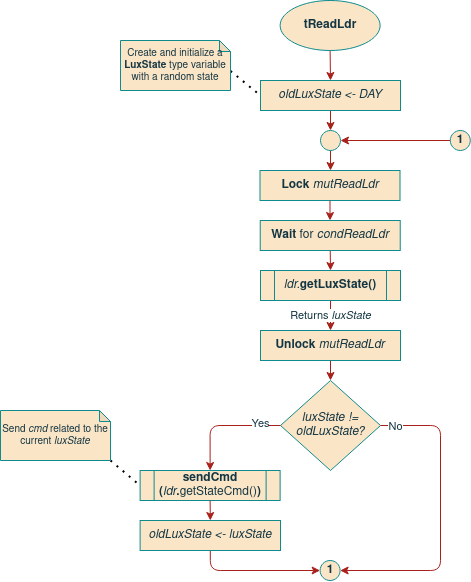
\includegraphics[width=.3\textwidth]{09sw_specification/LS/csensors/treadldr}
	\caption{Flowchart: CSensors tReadLdr method.}
	\label{fig:CSensorstreadldr}
\end{figure}

%******************************
aaaaaaaaaaaaaaa

\begin{figure}[H]
	\centering
	%	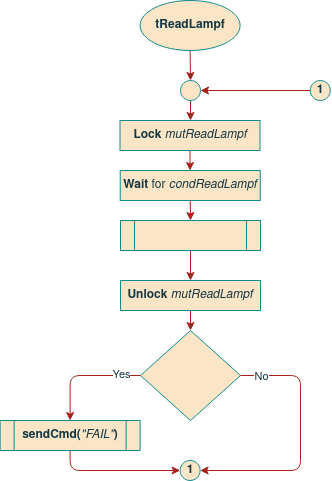
\includegraphics[width=.3\textwidth]{09sw_specification/LS/csensors/treadlampf}
	\caption{Flowchart: CSensors tReadLampf method.}
	\label{fig:CSensorstreadlampf}
\end{figure}

%******************************
The method \textit{sendCmd}, shown in figure \ref{fig:CSensorssendcmd}, is responsible for sending a string, \textit{cmd}, to the message queue, \textit{msgqSensors}. After that, it sends a signal, \textit{SIGUSR1}, to the process \textit{mainPID}, which is the main process PID.

\begin{figure}[H]
	\centering
	%	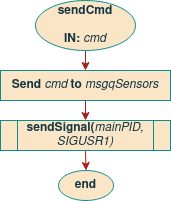
\includegraphics[width=.3\textwidth]{09sw_specification/LS/csensors/sendcmd}
	\caption{Flowchart: CSensors sendCmd method.}
	\label{fig:CSensorssendcmd}
\end{figure}

%******************************
The method \textit{PirISR}, is executed when there is motion detected, sending the \textit{"ON"} command to the main process.

\begin{figure}[H]
	\centering
	%	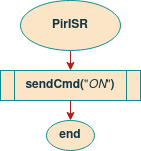
\includegraphics[width=.3\textwidth]{09sw_specification/LS/csensors/pirisr}
	\caption{Flowchart: CSensors PirISR method.}
	\label{fig:CSensorspirisr}
\end{figure}

%**********************************************************
\clearpage
\myparagraph{CCommunication Methods}

The class constructor is shown in figure \ref{fig:CCommunicationConstructor}. This is responsible for initializing all synchronization tools and private variables used.

\begin{figure}[H]
	\centering
%	\includegraphics[width=.3\textwidth]{09sw_specification/LS/ccommunication/constructor}
	\caption{Flowchart: CCommunication constructor.}
	\label{fig:CCommunicationConstructor}
\end{figure}

%******************************
To send a message, this class has a built-in thread, \textit{tSend} that can be created using \textit{init(tprio)}, which expects a priority for the thread, \textit{tprio}, as shown in figure \ref{fig:CCommunicationinit}.

\begin{figure}[H]
	\centering
	%	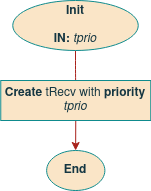
\includegraphics[width=.25\textwidth]{09sw_specification/LS/ccommunication/init}
	\caption{Flowchart: CCommunication Init method.}
	\label{fig:CCommunicationinit}
\end{figure}

%******************************
A message can be put in the waiting list to be sent through the use of \textit{push(msg)}, as shown in figure \ref{fig:CCommunicationPush}. This function is responsible for adding a new message, \textit{msg}, to the \textit{TxMsgs} vector, and signal the condition variable \textit{condSend}, for the thread \textit{tSend} to send the message.

\begin{figure}[H]
	\centering
%	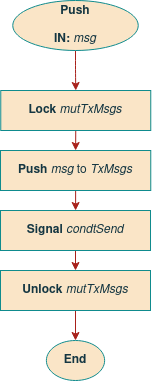
\includegraphics[width=.3\textwidth]{09sw_specification/LS/ccommunication/push}
	\caption{Flowchart: CCommunication Push method.}
	\label{fig:CCommunicationPush}
\end{figure}

%******************************
This thread, \textit{tSend} presented in figure \ref{fig:CCommunicationtsend}, is responsible for sending queued messages to the gateway, using LoRa communication. A conditional variable is used to wake this thread when there is a new message available to be sent.

When the queue \textit{TxMsgs} is empty, the task goes to sleep, waiting for the condition variable \textit{condSend} to notify this task. After this, the mutex \textit{mutComms} is used to protect the communication. Then, a message is popped from the messages queue, and sent to the gateway using the method \textit{Send}, shown in figure \ref{fig:CCommunicationsend}. This continues to happen until the \textit{TxMsgs} queue gets empty.

\begin{figure}[H]
	\centering
%	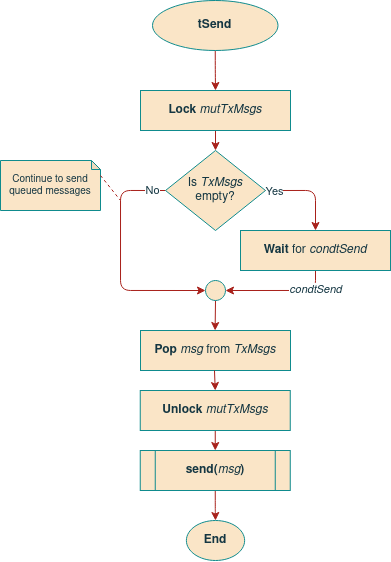
\includegraphics[width=.65\textwidth]{09sw_specification/LS/ccommunication/tsend}
	\caption{Flowchart: CCommunication tSend thread.}
	\label{fig:CCommunicationtsend}
\end{figure}

\begin{figure}[H]
	\centering
%	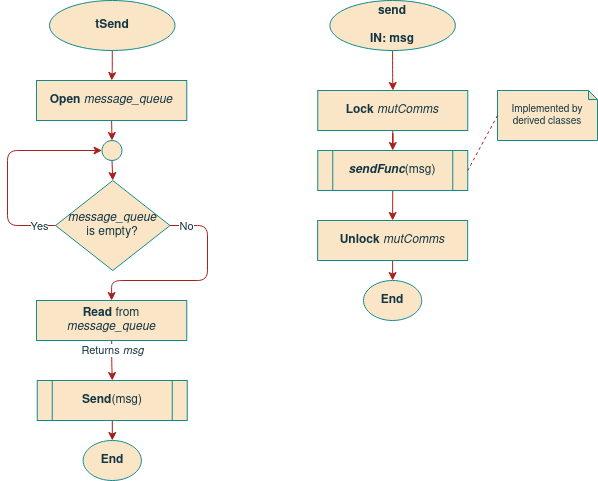
\includegraphics[width=.55\textwidth]{09sw_specification/LS/ccommunication/send}
	\caption{Flowchart: CCommunication Send method.}
	\label{fig:CCommunicationsend}
\end{figure}

%******************************
There is also another method, \textit{recv()}, that receives a message from the gateway, in a non blocking mode, making use of task synchronization tools to ensure that sending and receiving don't occur at the same time. This function should be used continuously if one doesn't want to miss any communication. This method is presented in figure \ref{fig:CCommunicationrecv}.

\begin{figure}[H]
	\centering
%	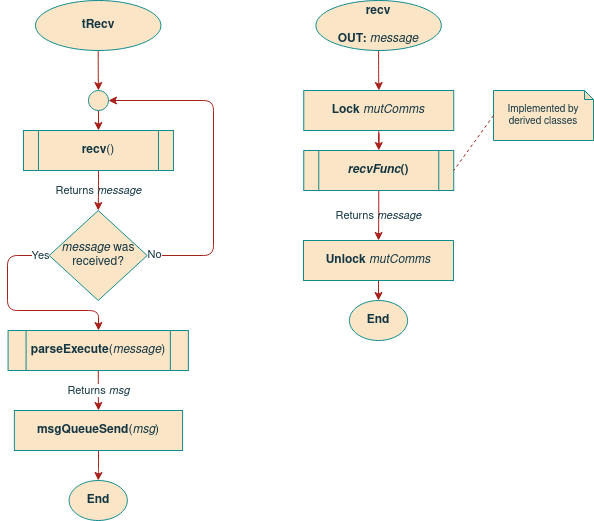
\includegraphics[width=.5\textwidth]{09sw_specification/LS/ccommunication/recv}
	\caption{Flowchart: CCommunication Recv method.}
	\label{fig:CCommunicationrecv}
\end{figure}

%**********************************************************
\clearpage
\myparagraph{CLoraComm Methods}

A CLoraComm object can be created through the use of the constructor, as shown in figure \ref{fig:LoraComm}.
This starts by initializing the LoRa communication, using the given frequency, \textit{freq}, which will be 433~MHz, and defining the pins connected to the module. At the end, all private members are also initialized.

\begin{figure}[H]
	\centering
%	\includegraphics[width=.6\textwidth]{09sw_specification/LS/cloracomm/constructor}
	\caption{Flowchart: CLoraComm constructor.}
	\label{fig:LoraComm}
\end{figure}

This class inherits from \textit{CCommunication} class, so this must implement \textit{recvFunc} and \textit{sendFunc}, as they are pure virtual methods. In this class, one will use existent functions \textit{LoraReceive} and \textit{LoraSend} to implement Lora communication, as shown in figures \ref{fig:CLoraCommrecvfunc} and \ref{fig:CLoraCommsendfunc}. This functions make use of the address of the local system, \textit{local\_addr}, defining the source ID, and the address of the gateway, \textit{dest\_addr}, defining the destination ID.

\begin{figure}[H]
	\centering
	%	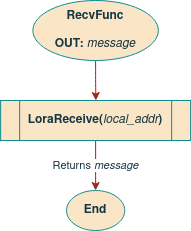
\includegraphics[width=.6\textwidth]{09sw_specification/LS/cloracomm/recvfunc}
	\caption{Flowchart: CLoraComm recvFunc method.}
	\label{fig:CLoraCommrecvfunc}
\end{figure}

\begin{figure}[H]
	\centering
	%	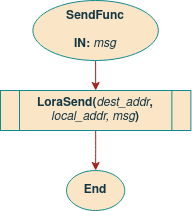
\includegraphics[width=.6\textwidth]{09sw_specification/LS/cloracomm/sendfunc}
	\caption{Flowchart: CLoraComm sendFunc method.}
	\label{fig:CLoraCommsendfunc}
\end{figure}


%**********************************************************
\clearpage
\myparagraph{CLamp Methods}

A CLamp object can be created or destroyed through the class constructor or destroyer, presented in figure \ref{fig:CLampconstructor}. When creating an object, one must pass to the constructor the time from which the lamp will stay on after one sets the brightness to the maximum. This value must be in seconds and is stored in the variable \textit{LampOnTimeoutSecs}.

\begin{figure}[H]
	\centering	
	%	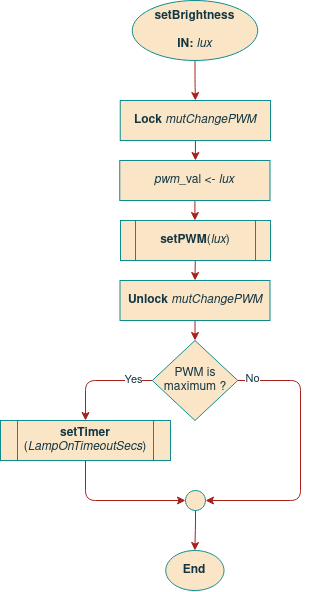
\includegraphics[width=.6\textwidth]{09sw_specification/clamp/setbrightness}
	\caption{Flowchart: CLamp constructor and destroyer.}
	\label{fig:CLampconstructor}
\end{figure}

%******************************
This function, presented in figure \ref{fig:CLampsetBrightness}, is responsible for changing the PWM associated with the lamp, which is directly related to its brightness.

Through \textit{setPWM(lux)} one can change the applied lamp PWM to \textit{lux} value, being this an integer between 0 to 100. When the PWM is maximum, a timer is started that defines how much time the lamp is ON, \textit{LampOnTimeoutSecs} in seconds.

\begin{figure}[H]
	\centering	
	%	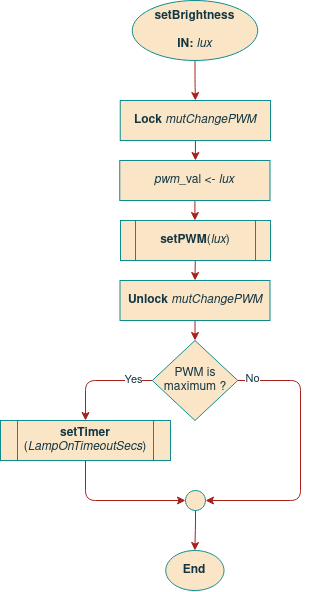
\includegraphics[width=.6\textwidth]{09sw_specification/clamp/setbrightness}
	\caption{Flowchart: CLamp setBrightness method.}
	\label{fig:CLampsetBrightness}
\end{figure}

%**********************************************************
\clearpage
\myparagraph{CParkDetection Methods}

In the method \textit{calcVacantsNum()}, one receives an image frame and processes it in order to determine the number of available parking spots. This does the detection of cars using a pre-trained model. When analyzing the image, if the coordinates of a detected car matches the coordinates of the parking spot (i.e the parking outline, obtained by \textit{getOutline()}) then one can assume that the parking spot is occupied. \\

%******************************
This method, represented in figure \ref{fig:CParkDetectiongetoutline}, is used to process the image captured by the camera in order to detect the parking spots outline. This is done using the algorithm defined previously in the section \ref{section:imageProc}, and starts by converting the frame to a grey scale image, apply the canny edge filter to highlight the edges of the image captured. After having the edges, one can select only the vertical and horizontal straight lines and intersect them, storing the intersection points, that are the parking spot coordinates, into the private member \textit{parkCoords}.

\begin{figure}[H]
	\centering			
	%	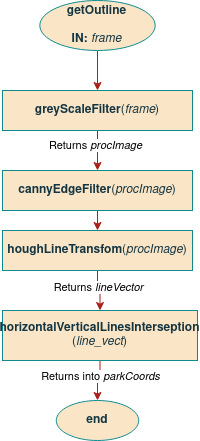
\includegraphics[width=.5\textwidth]{09sw_specification/cparkdetection/getoutline}
	\caption{Flowchart: CParkDetection getOutline method.}
	\label{fig:CParkDetectiongetoutline}
\end{figure}

%**********************************************************
\clearpage
\myparagraph{CLdr Methods}

The constructor for the class \textit{CLdr} is presented in \ref{fig:CLdrconstructor}. This creates an \textit{CLdr} object, initializing the LDR sensor, defining the initial luminosity state, \textit{luxState} and defining the command list for this sensor.

\begin{figure}[H]
	\centering
	%	\includegraphics[width=.7\textwidth]{09sw_specification/LS/cldr/constructor}
	\caption{Flowchart: CLdr constructor.}
	\label{fig:CLdrconstructor}
\end{figure}

%******************************
In order to obtain the current luminosity state, \textit{DAY} or \textit{NIGHT}, there is a method called \textit{getLuxState}, presented in figure \ref{fig:CLdrgetLuxState}. This method, gets the sensed luminosity level from the LDR sensor, and determines the current luminosity state.

\begin{figure}[H]
	\centering
	%	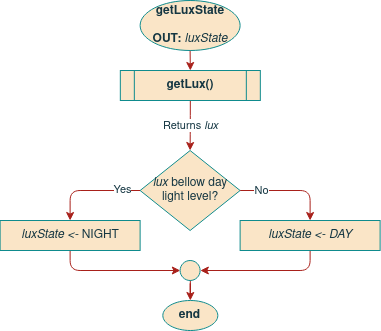
\includegraphics[width=.7\textwidth]{09sw_specification/LS/cldr/getluxstate}
	\caption{Flowchart: CLdr getLuxState method.}
	\label{fig:CLdrgetLuxState}
\end{figure}

%******************************
Depending on the luminosity state, \textit{luxState}, the CLdr must send a different command, when required to do so. Using the class command list and the variable \textit{luxState} one can obtain the command related to the current luminosity state, as shown in figure \ref{fig:CLdrgetStateCmd}.

\begin{figure}[H]
	\centering
	%	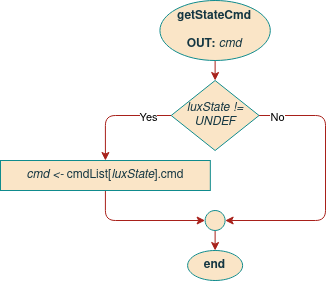
\includegraphics[width=.7\textwidth]{09sw_specification/LS/cldr/getstatecmd}
	\caption{Flowchart: CLdr getStateCmd method.}
	\label{fig:CLdrgetStateCmd}
\end{figure}

%**********************************************************
\clearpage
\myparagraph{CPir Methods}

In figure \ref{fig:CPirconstructor} is shown the CPir class constructor. This creates a CPir object, by firstly inserting the respective device driver, which will be developed, as a constraint of this project. Then an ISR is assigned to the PIR sensor, being that defined by a function pointer passed by argument into the constructor. Whenever the PIR detects movement in the surroundings, the output pin will change its value, triggering an interrupt, handled by the defined ISR.

\begin{figure}[H]
	\centering
	%	\includegraphics[width=.7\textwidth]{09sw_specification/LS/cpir/constructor}
	\caption{Flowchart: CPir constructor.}
	\label{fig:CPirconstructor}
\end{figure}


